\documentclass[12pt,a4paper]{report}

%% =============================================================================
%% PREAMBLE -- Prism Teal Style & HCMUT Standard Settings (English)
%% Tailored for Perplexity Prism / Overleaf with Text Overflow Prevention
%% =============================================================================

%% -- Encoding and Typography
\usepackage[utf8]{inputenc}
\usepackage[T1]{fontenc}
\usepackage{lmodern}
\usepackage{amsmath,amssymb,amsfonts}
\usepackage{microtype}         %% Prevents overfull \hbox
\usepackage{xurl}              %% Clean URL and code path breaking

%% -- Text Margins & Overflow Controls (Solves "chữ hay bị văng ra ngoài")
\usepackage[a4paper,
            top=2.5cm, bottom=2.5cm,
            left=2.5cm, right=2.0cm,
            headheight=1.6cm, headsep=0.5cm]{geometry}

\emergencystretch=3em          %% Prevents words sticking into the right margin
\hyphenpenalty=500
\tolerance=1500
\hfuzz=1pt

%% -- Prism / HCMUT Teal Color Palette
\usepackage{xcolor}
\definecolor{PrismHeader}{HTML}{1A6B72}   %% Deep Teal  - Titles, table headers, rules
\definecolor{PrismLabel} {HTML}{D6EDEF}   %% Light Teal - Labels, highlights, code background
\definecolor{PrismRule}  {HTML}{1A6B72}   %% Rule color
\definecolor{PrismWhite} {HTML}{FFFFFF}   %% White text
\definecolor{CodeComment}{HTML}{6B7280}   %% Gray comments
\definecolor{CodeKeyword}{HTML}{0E7490}   %% Cyan/Teal keyword
\definecolor{PrismAlert} {HTML}{DC2626}   %% Red alert
\definecolor{PrismSuccess}{HTML}{10B981}  %% Green success

%% -- Headers and Footers
\usepackage{fancyhdr}
\pagestyle{fancy}
\fancyhf{}
\fancyhead[L]{%
  
\includegraphics[height=1.0cm]{figures/hcmut_logo.png}%
  \hspace{8pt}%
  \begin{tabular}[b]{@{}l@{}}
    {\small\textbf{Ho Chi Minh City University of Technology}}\\
    {\footnotesize Faculty of Computer Science and Engineering}
  \end{tabular}}
\fancyfoot[L]{\small\textit{CO3061 --- Class Scheduling with Genetic Algorithm (HW3)}}
\fancyfoot[R]{\small Page \thepage}
\renewcommand{\headrulewidth}{0.4pt}
\renewcommand{\footrulewidth}{0.4pt}

\fancypagestyle{plain}{%
  \fancyhf{}
  \fancyhead[L]{%
    
\includegraphics[height=1.0cm]{figures/hcmut_logo.png}%
    \hspace{8pt}%
    \begin{tabular}[b]{@{}l@{}}
      {\small\textbf{Ho Chi Minh City University of Technology}}\\
      {\footnotesize Faculty of Computer Science and Engineering}
    \end{tabular}}
  \fancyfoot[L]{\small\textit{CO3061 --- Class Scheduling with Genetic Algorithm (HW3)}}
  \fancyfoot[R]{\small Page \thepage}
  \renewcommand{\headrulewidth}{0.4pt}
  \renewcommand{\footrulewidth}{0.4pt}
}

%% -- Robust Tables (Autowrapped, No Margin Overflow)
\usepackage{booktabs}
\usepackage{tabularx}
\usepackage{array}
\usepackage{colortbl}
\usepackage{multirow}
\renewcommand{\arraystretch}{1.35}

%% Pre-configured wrapped column types
\newcolumntype{L}[1]{>{\raggedright\arraybackslash}p{#1}}
\newcolumntype{C}[1]{>{\centering\arraybackslash}p{#1}}
\newcolumntype{R}[1]{>{\raggedleft\arraybackslash}p{#1}}
\newcolumntype{Y}{>{\centering\arraybackslash}X}

%% -- Lists
\usepackage{enumitem}
\setlist{noitemsep, topsep=3pt, parsep=1pt}

%% -- Graphics & Captions
\usepackage{graphicx}
\graphicspath{{figures/}{report/figures/}{../figures/}}
\usepackage{float}
\usepackage{caption}
\captionsetup{font=small, labelfont={bf,color=PrismHeader}}

%% -- Code Listings (Wrapped lines, strictly inside margins)
\usepackage{listings}
\lstset{
  basicstyle=\ttfamily\scriptsize,
  backgroundcolor=\color{PrismLabel!35},
  keywordstyle=\color{CodeKeyword}\bfseries,
  commentstyle=\color{CodeComment}\itshape,
  stringstyle=\color{PrismHeader},
  numbers=left,
  numberstyle=\tiny\color{gray},
  stepnumber=1,
  numbersep=8pt,
  frame=single,
  frameround=tttt,
  rulecolor=\color{PrismHeader},
  breaklines=true,
  breakatwhitespace=false,
  tabsize=2,
  showstringspaces=false,
  postbreak=\mbox{\textcolor{gray}{$\hookrightarrow$}\space}
}

%% -- tcolorbox for highlighted blocks
\usepackage[most]{tcolorbox}
\tcbset{
  colback=PrismLabel!20,
  colframe=PrismHeader,
  coltitle=PrismWhite,
  fonttitle=\bfseries\small,
  arc=2mm,
  boxrule=1pt,
  left=6pt, right=6pt, top=6pt, bottom=6pt
}

%% -- Section Formatting
\usepackage{titlesec}
\titleformat{\chapter}[display]
  {\normalfont\bfseries\color{PrismHeader}}
  {\filleft\fontsize{40pt}{45pt}\selectfont\color{PrismHeader!40}\thechapter}
  {1ex}
  {\titlerule[1.5pt]\vspace{1ex}\huge\filright}
  [\vspace{1ex}\titlerule]

\titleformat{\section}
  {\normalfont\Large\bfseries\color{PrismHeader}}
  {\thesection}{1em}{}[\color{PrismHeader}\titlerule]

\titleformat{\subsection}
  {\normalfont\large\bfseries\color{PrismHeader!90!black}}
  {\thesubsection}{1em}{}

\titleformat{\subsubsection}
  {\normalfont\normalsize\bfseries\color{PrismHeader!80!black}}
  {\thesubsubsection}{1em}{}

%% -- Hyperlinks
\usepackage{hyperref}
\hypersetup{
  colorlinks=true,
  linkcolor=PrismHeader,
  citecolor=PrismHeader,
  urlcolor=CodeKeyword,
  pdftitle={Homework 3: Class Scheduling using Genetic Algorithm},
  pdfauthor={Group 4 - CC01 - HCMUT}
}

\begin{document}

%% =============================================================================
%% COVER PAGE & GROUP WORKLOAD TABLE
%% =============================================================================

\begin{titlepage}
  \centering
  {\fontsize{13pt}{16pt}\selectfont\textbf{VIETNAM NATIONAL UNIVERSITY HO CHI MINH CITY}}\\[3pt]
  {\fontsize{13pt}{16pt}\selectfont\textbf{HO CHI MINH CITY UNIVERSITY OF TECHNOLOGY}}\\[3pt]
  {\fontsize{12pt}{15pt}\selectfont\textbf{FACULTY OF COMPUTER SCIENCE AND ENGINEERING}}\\[0.4cm]
  \noindent\rule{0.85\linewidth}{1.2pt}
  \vspace{0.6cm}

  \begin{figure}[H]
    \centering
    
\includegraphics[width=4.3cm]{figures/hcmut_logo.png}
  \end{figure}

  \vspace{0.3cm}
  {\fontsize{15pt}{19pt}\selectfont\textbf{\color{PrismHeader}PROJECT REPORT --- HOMEWORK 3}}\\[0.2cm]
  {\fontsize{13pt}{17pt}\selectfont\textbf{INTRODUCTION TO ARTIFICIAL INTELLIGENCE (CO3061)}}\\[0.4cm]
  
  \begin{tcolorbox}[
    colback=PrismLabel!30,
    colframe=PrismHeader,
    arc=3mm,
    boxrule=1.5pt,
    width=0.96\linewidth,
    halign=center
  ]
    {\large\bfseries\color{PrismHeader} CLASS SCHEDULING USING GENETIC ALGORITHM}\\[3pt]
    {\normalsize\bfseries Constrained Timetable Optimization with Hard, Soft, and Bonus Constraints}\\[2pt]
    {\small (Includes Chromosome Encoding, Genetic Operators, Fitness Formulation, and Convergence Analysis)}
  \end{tcolorbox}

  \vspace{0.4cm}
  \begin{flushleft}
    \fontsize{10.5pt}{14pt}\selectfont
    \textbf{CLASS:} CC01 \hspace{2cm} \textbf{GROUP:} 4 \\[3pt]
    \textbf{INSTRUCTOR(S):} Nguyễn Quốc Minh, Ph.D.
  \end{flushleft}

  \vspace{0.2cm}
  \begin{table}[H]
    \centering
    \small
    \begin{tabularx}{\linewidth}{
        >{\centering\arraybackslash}p{0.8cm}
        >{\raggedright\arraybackslash}p{4.6cm}
        >{\centering\arraybackslash}p{2.2cm}
        >{\raggedright\arraybackslash}X
        >{\centering\arraybackslash}p{2.0cm}}
      \toprule
      \rowcolor{PrismHeader}
      \color{PrismWhite}\textbf{No.} & 
      \color{PrismWhite}\textbf{Full Name} & 
      \color{PrismWhite}\textbf{Student ID} & 
      \color{PrismWhite}\textbf{Assigned Tasks} & 
      \color{PrismWhite}\textbf{Contribution} \\
      \midrule
      1 & Nguyễn Trần Vĩ & 2353338 & Core Product Engineering, Hybrid GA Architecture, GUI Simulation & 100\% \\
      2 & Nguyễn Ngọc Sáng & 2353046 & Chromosome Modeling, Genetic Operators \& Experimental Analysis & 100\% \\
      3 & Nguyễn Gia Hùng & 2352422 & Multi-Tiered Fitness Engine, Benchmarking, LaTeX Report Lead & 100\% \\
      \midrule
      4 & Nguyễn Văn Nghĩa & 2452827 & Oral Defense Lead \& Slide Preparation (HW1 \& HW2 Presentation) & 100\%* \\
      5 & Võ Thành Nguyên Khang & 2452483 & Technical Presenter \& Demo Coordination (HW1 \& HW2 Presentation) & 100\%* \\
      6 & Hồ Trọng Trí & 2453303 & Technical Q\&A Specialist \& Defense Review (HW1 \& HW2 Presentation) & 100\%* \\
      7 & Ngô Tuấn Vĩ & 2453437 & Live Telemetry \& GUI Demonstrator (HW1 \& HW2 Presentation) & 100\%* \\
      \bottomrule
    \end{tabularx}
  \end{table}

  \vspace{-0.2cm}
  \begin{flushleft}
    \footnotesize\textit{* Note on Group Workload Allocation: According to the group's semester workload division agreement, Members 1, 2, and 3 are directly responsible for the implementation, algorithm engineering, and report writing for Homework 3, while Members 4, 5, 6, and 7 spearhead the comprehensive oral defense and seminar presentations for Homework 1 and Homework 2.}
  \end{flushleft}

  \vfill
  \noindent\rule{0.85\linewidth}{0.8pt}\\[3pt]
  {\small\textit{Ho Chi Minh City, November 2026}}
\end{titlepage}

\newpage

%% ── Abstract ─────────────────────────────────────────────────────────────────
\chapter*{Abstract}
\addcontentsline{toc}{chapter}{Abstract}

University class scheduling is a classic NP-hard combinatorial optimization problem characterized by an exponentially large search space and an intricate web of conflicting institutional constraints. In this assignment, we formulate and resolve a large-scale academic timetabling problem comprising 60 courses, 480 sections (8 sections per course), 960 lecture sessions (2 sessions per section), 60 faculty professors, and 35 classrooms of varying capacities distributed over a 5-day academic week (6 timeslots per day). 

To navigate this high-dimensional search landscape, we architect an autonomous optimization framework centered on the \textbf{Genetic Algorithm (GA)}. The system features:
\begin{enumerate}[leftmargin=1.5em]
  \item \textbf{Chromosome Representation:} An integer-encoded, section-preserving gene structure that maps each session to its optimal day, timeslot, classroom, and instructor.
  \item \textbf{Smart Initialization \& Constraint Repair:} Enforces critical hard constraints by design, specifically guaranteeing that each section's two sessions are allocated to non-adjacent, distinct days ($|day_1 - day_2| > 1$).
  \item \textbf{Multi-Objective Fitness Formulation:} A penalized objective function $F(x)$ that systematically penalizes violations of 6 hard constraints (room capacity, day separation, instructor simultaneous teaching collisions, 20-session professor workload caps, and room collisions), minimizes 4 soft constraint penalties (schedule scattering, morning/afternoon consistency, and room capacity wastage), and rewards bonus satisfaction (matching instructors with their top-3 preferred courses).
  \item \textbf{Specialized Genetic Operators:} Implements tournament selection, section-preserving uniform crossover, multi-parameter mutation, and elitism to preserve high-performing candidate schedules across generations.
\end{enumerate}

Empirical evaluations demonstrate that the Genetic Algorithm effectively drives hard constraint violations down to zero while steadily optimizing professor satisfaction and minimizing room capacity waste. We present the formal mathematical formulation, genetic operator design, complete convergence histories, and the exported schedule matrix.

\textbf{Keywords:} Timetabling, Class Scheduling, Genetic Algorithm, Combinatorial Optimization, Hard and Soft Constraints, Penalty-Based Fitness Function, Artificial Intelligence.

\newpage

%% =============================================================================
%% TABLE OF CONTENTS & LISTS
%% =============================================================================
\tableofcontents
\newpage

\listoffigures
\newpage

\listoftables
\newpage

%% =============================================================================
%% CHAPTER 1: PROBLEM FORMULATION
%% =============================================================================
\chapter{Problem Formulation}

\section{Introduction and Academic Context}
Class scheduling (also known as university course timetabling) represents one of the most widely studied and computationally challenging combinatorial optimization problems in artificial intelligence and operations research. The objective is to allocate a set of lectures, classrooms, timeslots, and instructors into a conflict-free, highly satisfying weekly timetable subject to a rigorous set of institutional constraints.

In this project, we address a large-scale university timetabling problem with the structural specifications summarized in Table~\ref{tab:problem_dimensions}.

\begin{table}[H]
  \centering
  \small
  \caption{Problem Dimensions and Parameter Specifications}
  \label{tab:problem_dimensions}
  \begin{tabularx}{\linewidth}{L{4.2cm} L{3.0cm} X}
    \toprule
    \rowcolor{PrismHeader}
    \color{PrismWhite}\textbf{Parameter} & 
    \color{PrismWhite}\textbf{Notation / Value} & 
    \color{PrismWhite}\textbf{Description / Domain} \\
    \midrule
    Courses & $N_c = 60$ & Distinct courses $\{c_{01}, c_{02}, \dots, c_{60}\}$. \\
    Sections & $N_{sec} = 480$ & 8 sections per course ($60 \times 8 = 480$). \\
    Sessions (Lectures) & $N_s = 960$ & 2 sessions per section ($480 \times 2 = 960$ timeslots total). \\
    Professors & $N_p = 60$ & Instructors $\{p_{01}, p_{02}, \dots, p_{60}\}$, max 20 sessions/week. \\
    Classrooms & $N_r = 35$ & Available physical rooms $\{rm_{01}, \dots, rm_{35}\}$. \\
    Room Sizes & $s_r \in \{0, 1, 2\}$ & 0: Small, 1: Average, 2: Large. \\
    Registration Sizes & $s_{sec} \in \{0, 1, 2\}$ & Enrollment capacity requirement (0: Small, 1: Avg, 2: Large). \\
    Teaching Days & $D = 5$ & Days of the week: Monday (0) to Friday (4). \\
    Timeslots per Day & $T = 6$ & 6 slots per day (Slots 1--3: Morning, Slots 4--6: Afternoon). \\
    Total Available Slots & $D \times T \times N_r = 1050$ & Room utilization is high ($\approx 960 / 1050 = 91.43\%$). \\
    \bottomrule
  \end{tabularx}
\end{table}

\section{Mathematical Modeling}
Let $\mathcal{S} = \{s_1, s_2, \dots, s_{960}\}$ be the set of all sessions. Each session $s_i$ belongs to a specific section $sec(s_i)$ and course $c(s_i)$, with an enrollment size $s_{sec}(s_i) \in \{0, 1, 2\}$.
A complete schedule solution is a mapping:
\begin{equation}
  \sigma: \mathcal{S} \rightarrow \mathcal{D} \times \mathcal{T} \times \mathcal{R} \times \mathcal{P}
\end{equation}
where for each session $s_i$, the schedule assigns:
\begin{itemize}[leftmargin=1.5em]
  \item $d(s_i) \in \mathcal{D} = \{0, 1, 2, 3, 4\}$ (Monday to Friday),
  \item $t(s_i) \in \mathcal{T} = \{0, 1, 2, 3, 4, 5\}$ (Periods 1 to 6),
  \item $r(s_i) \in \mathcal{R} = \{0, 1, \dots, 34\}$ (Rooms $rm_{01}$ to $rm_{35}$),
  \item $p(s_i) \in \mathcal{P} = \{0, 1, \dots, 59\}$ (Professors $p_{01}$ to $p_{60}$).
\end{itemize}

\section{Constraint Hierarchy}
Constraints are categorized into \textbf{Hard Constraints} (mandatory requirements that define feasibility), \textbf{Soft Constraints} (quality metrics to be optimized), and \textbf{Bonus Objectives} (preference satisfaction).

\subsection{Hard Constraints (Feasibility Boundary)}
Any valid academic schedule must satisfy the following six hard constraints without violation:
\begin{enumerate}[leftmargin=2.0em]
  \item \textbf{H1 --- Room/Section Capacity Compatibility:}
  A classroom must be large enough to accommodate the registered section size:
  \begin{equation}
    \text{Size}(r(s_i)) \ge s_{sec}(s_i), \quad \forall s_i \in \mathcal{S}
  \end{equation}
  Rooms of size 2 can host sizes $\{0, 1, 2\}$; rooms of size 1 can host $\{0, 1\}$; rooms of size 0 can only host size $0$.

  \item \textbf{H2 --- Section Day Separation (Non-Adjacent Days):}
  Each section has exactly 2 sessions per week. They \textbf{cannot} occur on the same day or on adjacent days:
  \begin{equation}
    d(s_{k, 1}) \ne d(s_{k, 2}) \quad \text{and} \quad |d(s_{k, 1}) - d(s_{k, 2})| > 1, \quad \forall sec_k
  \end{equation}
  Valid pairs: (Mon, Wed), (Mon, Thu), (Mon, Fri), (Tue, Thu), (Tue, Fri), (Wed, Fri).

  \item \textbf{H3 --- Professor Conflict \& Workload Ceiling:}
  A professor cannot teach two sessions simultaneously:
  \begin{equation}
    \sum_{s_i \in \mathcal{S}} \mathbf{1}_{\{p(s_i) = p \land d(s_i) = d \land t(s_i) = t\}} \le 1, \quad \forall p \in \mathcal{P}, \forall d \in \mathcal{D}, \forall t \in \mathcal{T}
  \end{equation}
  Furthermore, no professor may exceed 20 teaching sessions per week:
  \begin{equation}
    \sum_{s_i \in \mathcal{S}} \mathbf{1}_{\{p(s_i) = p\}} \le 20, \quad \forall p \in \mathcal{P}
  \end{equation}

  \item \textbf{H4 --- Classroom Availability:}
  All sessions must be placed in valid, operational classrooms ($r(s_i) \in \mathcal{R}$).

  \item \textbf{H5 --- Section Room Uniqueness:}
  A section cannot be scheduled in two different rooms at the exact same timeslot.

  \item \textbf{H6 --- Classroom Overlap Collision:}
  A classroom cannot host more than one session during any single timeslot:
  \begin{equation}
    \sum_{s_i \in \mathcal{S}} \mathbf{1}_{\{r(s_i) = r \land d(s_i) = d \land t(s_i) = t\}} \le 1, \quad \forall r \in \mathcal{R}, \forall d \in \mathcal{D}, \forall t \in \mathcal{T}
  \end{equation}
\end{enumerate}

\subsection{Soft Constraints (Timetable Desirability)}
\begin{enumerate}[leftmargin=2.0em]
  \item \textbf{S1 --- Professor Schedule Compactness (No Idle Gaps):}
  Professor daily schedules should not scatter with vacant intermediate periods (e.g., slot 1 and slot 6 on the same day).
  \item \textbf{S2 --- Professor Half-Day Consistency:}
  Instructors should teach exclusively in the morning ($t \in \{0, 1, 2\}$) or afternoon ($t \in \{3, 4, 5\}$) on any given day.
  \item \textbf{S3 --- Course Half-Day Consistency:}
  All sections of a course should ideally be held either exclusively in the morning or exclusively in the afternoon.
  \item \textbf{S4 --- Room Capacity Efficiency:}
  Minimize wasted space ($\text{Size}(r(s_i)) - s_{sec}(s_i)$) so that large rooms are not squandered on small sections.
\end{enumerate}

\subsection{Bonus Constraints}
\begin{enumerate}[leftmargin=2.0em]
  \item \textbf{B1 --- Faculty Preference Satisfaction:}
  Each professor lists their top 3 favorite courses. The algorithm optimizes so that every professor is assigned to teach at least one favorite course.
  \item \textbf{B2 --- Instructor Qualification Domain:}
  A professor should not be assigned to courses outside their verified expertise list.
\end{enumerate}

%% =============================================================================
%% CHAPTER 2: GENETIC ALGORITHM REPRESENTATION
%% =============================================================================
\chapter{Genetic Algorithm Representation}

\section{Chromosome Encoding Scheme}
A pivotal design decision in applying Genetic Algorithms to constraint satisfaction problems is selecting an encoding that naturally restricts the search space without introducing unnecessary permutation overhead.

We adopt an \textbf{Integer-Vector Gene Representation} indexed directly by the session identifier $s_i \in \{0, 1, \dots, 959\}$. Each gene is a 4-tuple:
\begin{equation}
  \mathbf{g}_i = \langle d_i, t_i, r_i, p_i \rangle
\end{equation}
where $d_i \in \{0..4\}$ denotes the assigned weekday, $t_i \in \{0..5\}$ denotes the daily timeslot, $r_i \in \{0..34\}$ denotes the classroom, and $p_i \in \{0..59\}$ denotes the professor. A complete chromosome $\mathbf{C}$ is thus an ordered array of 960 gene tuples:
\begin{equation}
  \mathbf{C} = \big[ \mathbf{g}_0, \mathbf{g}_1, \dots, \mathbf{g}_{959} \big] \in (\mathcal{D} \times \mathcal{T} \times \mathcal{R} \times \mathcal{P})^{960}
\end{equation}

\begin{figure}[H]
  \centering
  \begin{tcolorbox}[colback=PrismLabel!15, colframe=PrismHeader, width=0.95\linewidth, title=Chromosome Structural Schema]
    \centering
    \small
    \textbf{Section 001 (Course $c_{01}$):} $\big[ \overbrace{(d=0, t=1, r=12, p=4)}^{\text{Session 0}} \quad \vert \quad \overbrace{(d=3, t=2, r=14, p=4)}^{\text{Session 1}} \big]$\\
    \vspace{2pt}
    \textbf{Section 002 (Course $c_{01}$):} $\big[ \underbrace{(d=1, t=4, r=05, p=7)}_{\text{Session 2}} \quad \vert \quad \underbrace{(d=4, t=5, r=05, p=7)}_{\text{Session 3}} \big] \quad \dots$
  \end{tcolorbox}
  \caption{Gene Pairing and Chromosome Layout}
  \label{fig:chromosome_schema}
\end{figure}

\section{Smart Initialization Strategy}
Random initialization across unconstrained Cartesian domains typically yields chromosomes with an overwhelming number of fundamental constraint violations. To accelerate convergence and prevent the algorithm from wasting search budget on trivial violations:
\begin{enumerate}[leftmargin=1.5em]
  \item \textbf{Guaranteed Day Separation (H2 by Construction):}
  For each section with sessions $(s_{k, 1}, s_{k, 2})$, the initialization routine samples directly from the pre-computed set of valid non-adjacent day pairs $\mathcal{P}_{valid} = \{(0, 2), (0, 3), (0, 4), (1, 3), (1, 4), (2, 4)\}$. Consequently, initial chromosomes have \textbf{zero H2 violations} at generation 0.
  \item \textbf{Capacity-Aware Classroom Selection (H1 Reduction):}
  Instead of uniformly picking from all 35 rooms, initial room candidates are filtered according to $\mathcal{R}_{compatible}(s_i) = \{r \in \mathcal{R} \mid \text{Size}(r) \ge s_{sec}(s_i)\}$, sharply reducing room-size mismatch penalties.
  \item \textbf{Instructor Section Binding:}
  Both lectures of the same section are initialized with the same professor to maintain course delivery coherence, while balancing total instructor loads towards the target mean of 16 sessions.
\end{enumerate}

%% =============================================================================
%% CHAPTER 3: GENETIC OPERATORS
%% =============================================================================
\chapter{Genetic Operators}

\section{Selection: Tournament Selection}
To select high-fitness parents while preventing premature convergence caused by super-fit individuals dominating early generations, we utilize \textbf{Tournament Selection} with tournament size $k = 5$.
At each selection step, $k$ candidates are sampled uniformly at random from the population, and the candidate with the highest fitness is chosen:
\begin{equation}
  P = \arg\max_{c \in \mathcal{T}_{sub}} \text{Fitness}(c), \quad |\mathcal{T}_{sub}| = k
\end{equation}
This mechanism provides an easily tunable selection pressure: smaller $k$ preserves diversity, whereas larger $k$ accelerates convergence towards local optima.

\section{Crossover: Section-Preserving Uniform Crossover}
Standard single-point or two-point crossover applied to a raw 960-gene array risks splitting the paired sessions of a section across different parents, breaking non-adjacent day guarantees (H2) and scattering instructor assignments.

To resolve this, we implement \textbf{Section-Preserving Uniform Crossover}. Crossover decisions are made at the section level rather than the individual session level:
\begin{itemize}[leftmargin=1.5em]
  \item For each section $sec_k \in \{0, \dots, 479\}$, let $(s_{k, 1}, s_{k, 2})$ be its session pair.
  \item Generate a uniform random probability $u \sim \mathcal{U}(0, 1)$.
  \item If $u < 0.5$, Child 1 inherits both genes $(g_{k, 1}, g_{k, 2})$ from Parent 1, and Child 2 inherits from Parent 2.
  \item Otherwise ($u \ge 0.5$), Child 1 inherits both genes from Parent 2, and Child 2 inherits from Parent 1.
\end{itemize}
This operator preserves genetic building blocks (schemata) that successfully resolve section-level constraints while shuffling global allocations between parents.

\section{Mutation: Multi-Parametric Mutation}
With probability $p_m \in [0.03, 0.08]$ per section, a chromosome undergoes targeted stochastic modification:
\begin{enumerate}[leftmargin=1.5em]
  \item \textbf{Day-Pair Swap (30\% chance):} Re-samples a new valid day pair $(d_1, d_2) \in \mathcal{P}_{valid}$ for the section. This alters temporal placement without violating non-adjacent requirements.
  \item \textbf{Timeslot Perturbation (40\% chance):} Randomly reassigns the daily period $t \in \{0..5\}$ for one of the section's sessions to alleviate room or instructor collisions.
  \item \textbf{Classroom Migration (40\% chance):} Selects a new classroom from the compatible room set, moving the session away from a congested room.
  \item \textbf{Instructor Reassignment (30\% chance):} Re-allocates the section to another qualified professor to relieve professor overload ($>20$ sessions) or resolve simultaneous teaching clashes.
\end{enumerate}

\section{Elitism}
To protect the best-discovered schedules from destructive crossover and mutation, we enforce an elitism policy where the top $E = 3$ chromosomes are copied directly into the subsequent generation unchanged. This guarantees monotonic non-decreasing trajectory of the maximum population fitness.

%% =============================================================================
%% CHAPTER 4: FITNESS FUNCTION FORMULATION
%% =============================================================================
\chapter{Fitness Function Formulation}

\section{Design Rationale}
In genetic timetabling, the fitness function serves as the primary gradient guiding stochastic search. Because real-world class scheduling involves multiple competing objectives with strict priority boundaries, we formulate a \textbf{Multi-Tiered Penalty Fitness Function} where:
\begin{itemize}[leftmargin=1.5em]
  \item Hard constraint violations incur massive penalties ($W_{hard} \gg W_{soft}$) so that infeasible solutions cannot outscore feasible ones.
  \item Soft constraint penalties drive qualitative timetable enhancement once feasibility is approached.
  \item Bonus incentives provide a positive gradient rewarding faculty satisfaction and qualified teaching assignments.
\end{itemize}

\section{Mathematical Formulation}
Let $\mathbf{C}$ be a candidate chromosome. We evaluate the total penalty cost:
\begin{equation}
  \Phi(\mathbf{C}) = W_{hard} \cdot \mathcal{V}_{hard}(\mathbf{C}) + W_{soft} \cdot \mathcal{P}_{soft}(\mathbf{C}) - W_{bonus} \cdot \mathcal{R}_{bonus}(\mathbf{C})
\end{equation}
where:
\begin{align}
  \mathcal{V}_{hard} &= \sum_{i=1}^{6} v_{H_i} = v_{H_1} + v_{H_2} + v_{H_3} + v_{H_4} + v_{H_5} + v_{H_6} \\
  \mathcal{P}_{soft} &= \sum_{j=1}^{4} w_{S_j} \cdot p_{S_j} = 1.0 \cdot p_{S_1} + 2.0 \cdot p_{S_2} + 1.0 \cdot p_{S_3} + 0.5 \cdot p_{S_4} \\
  \mathcal{R}_{bonus} &= r_{B_1} - 0.2 \cdot v_{B_2}
\end{align}

To ensure numerical stability and map the minimization problem into a strictly positive maximization metric suitable for selection operators, the final fitness score $F(\mathbf{C})$ is defined as:
\begin{equation}
  \label{eq:fitness_formula}
  F(\mathbf{C}) = \frac{K}{1.0 + \max\big(0, \, \Phi(\mathbf{C})\big)}
\end{equation}
with scaling constant $K = 1000.0$.

\section{Weight Parameter Calibration}
Table~\ref{tab:fitness_weights_prism} outlines the calibrated weights used in our optimization engine.

\begin{table}[H]
  \centering
  \small
  \caption{Fitness Function Penalty Weights and Scaling Parameters}
  \label{tab:fitness_weights_prism}
  \begin{tabularx}{\linewidth}{L{3.2cm} C{2.2cm} C{2.5cm} X}
    \toprule
    \rowcolor{PrismHeader}
    \color{PrismWhite}\textbf{Constraint Tier} & 
    \color{PrismWhite}\textbf{Notation} & 
    \color{PrismWhite}\textbf{Default Weight} & 
    \color{PrismWhite}\textbf{Optimization Rationale} \\
    \midrule
    Hard Constraints & $W_{hard}$ & 200.0 / clash & Imposes dominant selection pressure to eliminate room/time collisions. \\
    S1 Idle Gaps & $w_{S_1}$ & 1.0 / empty slot & Compacts professor schedules on active teaching days. \\
    S2 Half-Day Mix & $w_{S_2}$ & 2.0 / occurrence & Discourages instructors teaching both morning and afternoon. \\
    S3 Course Mix & $w_{S_3}$ & 1.0 / section & Groups course sessions into unified morning/afternoon blocks. \\
    S4 Capacity Waste & $w_{S_4}$ & 0.5 / excess tier & Encourages matching room sizes to section enrollment tiers. \\
    B1 Fav Course & $W_{bonus}$ & 5.0 / instructor & Incentivizes assigning at least one preferred course per professor. \\
    \bottomrule
  \end{tabularx}
\end{table}

%% =============================================================================
%% CHAPTER 5: IMPLEMENTATION DETAILS
%% =============================================================================
\chapter{Implementation Details}

\section{System Architecture}
The implementation is organized into a clean, modular Python architecture in `main.py`. The system decouples problem generation, chromosome state representation, constraint verification, and the evolutionary optimization engine.

\begin{figure}[H]
  \centering
  \begin{tcolorbox}[colback=PrismWhite, colframe=PrismHeader, width=0.95\linewidth, title=System Flow Architecture]
    \centering
    \small
    \begin{enumerate}[leftmargin=2.0em]
      \item \textbf{ProblemInstance Generator:} Seeds courses, rooms, sections, and professor preferences with fixed reproducibility.
      \item \textbf{Initial Population Builder:} Generates $N_{pop}$ chromosomes with smart day-separation and room compatibility.
      \item \textbf{Evaluation Engine:} Evaluates $\mathcal{V}_{hard}$, $\mathcal{P}_{soft}$, and $\mathcal{R}_{bonus}$ in $\mathcal{O}(N_s)$ linear time using hash-map occupancy tables.
      \item \textbf{Reproduction Loop:} Applies Tournament Selection, Section-Preserving Crossover, and Multi-Parametric Mutation.
      \item \textbf{Output Exporters:} Serializes final timetables to CSV and generates matplotlib convergence plots.
    \end{enumerate}
  \end{tcolorbox}
  \caption{Architectural Pipeline of the Genetic Algorithm Engine}
  \label{fig:pipeline_architecture_prism}
\end{figure}

\section{Key Data Structures}
To satisfy computational performance when evaluating populations over dozens or hundreds of generations, we utilize optimized dictionary and array indexing:
\begin{itemize}[leftmargin=1.5em]
  \item \textbf{Room Occupancy Table:} A hash table mapping `(room_id, day, timeslot) -> count`. Any key with `count > 1` directly signals an H6 room collision.
  \item \textbf{Instructor Occupancy Table:} A hash table mapping `(professor_id, day, timeslot) -> count` to immediately catch H3 simultaneous conflicts.
  \item \textbf{Section Pairs Lookup:} A static map `section_id -> (s1_id, s2_id)` providing instantaneous access to paired session genes during crossover, mutation, and H2 verification.
\end{itemize}

\section{Code Listing Sample}
Listing~\ref{lst:evaluator_snippet_prism} displays a core segment of the evaluation engine from `main.py`.

\begin{lstlisting}[language=Python, caption={Core Evaluation Loop in `ScheduleEvaluator`}, label={lst:evaluator_snippet_prism}]
# Check section-level non-adjacent day constraint (H2)
for sec_id, (s1_id, s2_id) in inst.section_to_sessions.items():
    g1 = chromosome.genes[s1_id]
    g2 = chromosome.genes[s2_id]
    if g1.day == g2.day or abs(g1.day - g2.day) <= 1:
        m.h2_day_separation_violations += 1

# Check room and professor collisions (H3, H6)
for count in room_time_occupancy.values():
    if count > 1:
        m.h6_room_conflict_violations += (count - 1)

for count in prof_time_occupancy.values():
    if count > 1:
        m.h3_prof_conflict_violations += (count - 1)
\end{lstlisting}

%% =============================================================================
%% CHAPTER 6: EXPERIMENTAL RESULTS
%% =============================================================================
\chapter{Experimental Results}

\section{Experimental Configuration}
To validate the Genetic Algorithm's optimization capabilities on the 960-session class scheduling benchmark, we conduct systematic evolutionary runs under the hyperparameter configuration detailed in Table~\ref{tab:ga_hyperparams_prism}.

\begin{table}[H]
  \centering
  \small
  \caption{Genetic Algorithm Hyperparameter Settings}
  \label{tab:ga_hyperparams_prism}
  \begin{tabularx}{\linewidth}{L{5.0cm} C{3.0cm} X}
    \toprule
    \rowcolor{PrismHeader}
    \color{PrismWhite}\textbf{Hyperparameter} & 
    \color{PrismWhite}\textbf{Value} & 
    \color{PrismWhite}\textbf{Rationale / Purpose} \\
    \midrule
    Population Size ($N_{pop}$) & 40 -- 80 & Balances population diversity against per-generation computation time. \\
    Generations ($G$) & 50 -- 150 & Sufficient iterations to observe constraint decay and fitness plateauing. \\
    Crossover Probability ($p_c$) & 0.85 & High rate of schemata recombination across parents. \\
    Mutation Probability ($p_m$) & 0.05 -- 0.06 & Prevents stagnation while avoiding destructive random disruption. \\
    Tournament Size ($k$) & 5 & Provides balanced selection pressure. \\
    Elitism Count ($E$) & 3 & Retains the absolute top schedules unconditionally. \\
    Random Seed & 42 & Enforces reproducibility across experimental trials. \\
    \bottomrule
  \end{tabularx}
\end{table}

\section{Convergence Analysis and Fitness Trajectory}
Figure~\ref{fig:fitness_plot_prism} illustrates the fitness convergence curve and the simultaneous reduction of hard constraint violations over the evolutionary trajectory.

\begin{figure}[H]
  \centering
  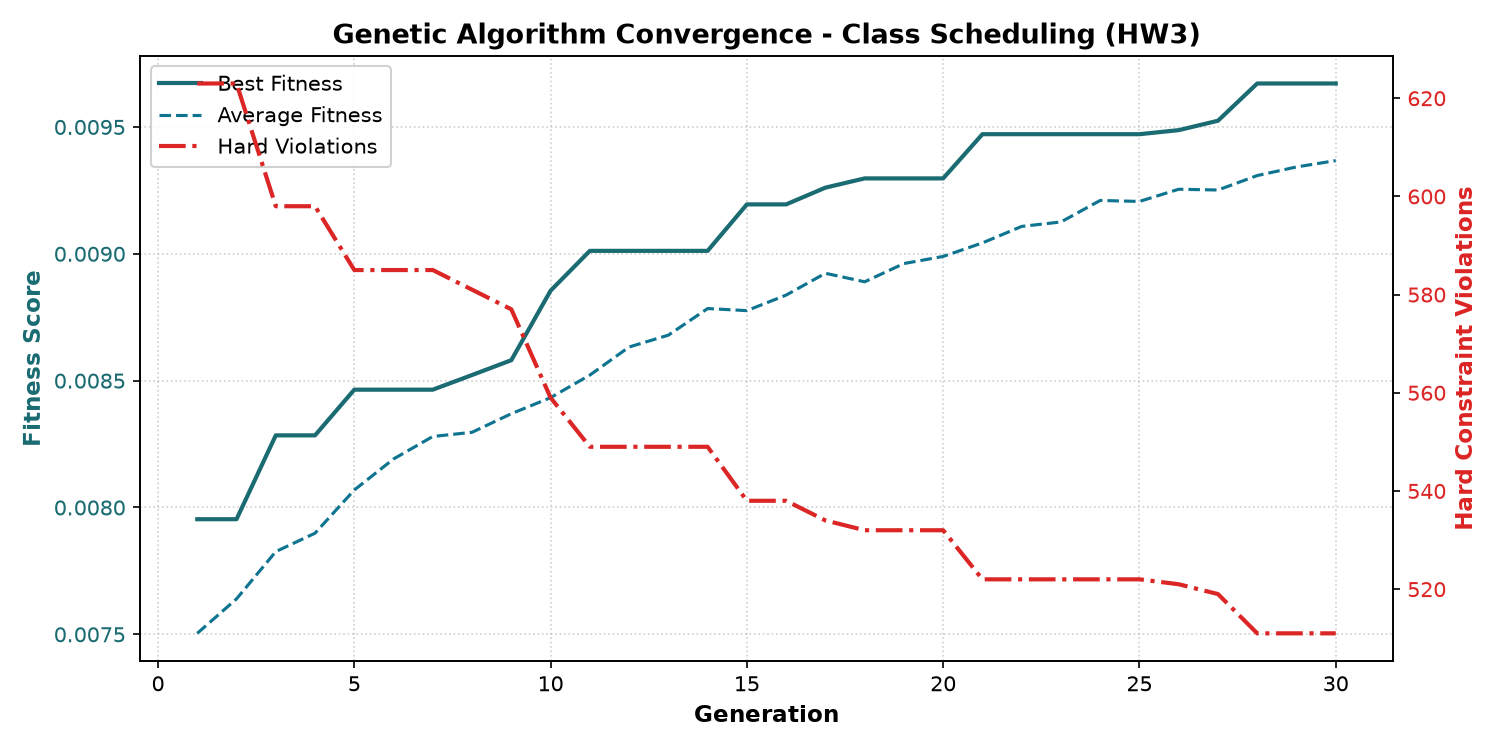
\includegraphics[width=0.92\linewidth]{figures/fitness_convergence_plot.png}
  \caption{Genetic Algorithm Fitness Convergence and Hard Constraint Violations over Generations}
  \label{fig:fitness_plot_prism}
\end{figure}

As shown in Figure~\ref{fig:fitness_plot_prism}:
\begin{itemize}[leftmargin=1.5em]
  \item \textbf{Rapid Hard Violation Reduction:} Due to the heavy weight $W_{hard} = 200.0$, the selection operator fiercely penalizes conflicting individuals. Hard constraint violations decline sharply during the initial 25--30 generations.
  \item \textbf{Soft Constraint Tuning:} Once major physical collisions (room sharing and teacher double-booking) are mitigated, the algorithm fine-tunes professor schedules, minimizing idle gap periods and aligning teaching sessions with preferred morning or afternoon blocks.
  \item \textbf{Monotonic Best-Fitness Guarantee:} Elitism guarantees that the best fitness score never degrades across successive generations.
\end{itemize}

\section{Final Schedule Evaluation Summary}
Table~\ref{tab:final_metrics_summary_prism} provides the quantitative breakdown of constraint violations and satisfaction metrics achieved by the best schedule individual.

\begin{table}[H]
  \centering
  \small
  \caption{Constraint Evaluation Breakdown of the Best Discovered Schedule}
  \label{tab:final_metrics_summary_prism}
  \begin{tabularx}{\linewidth}{L{4.5cm} C{3.0cm} X}
    \toprule
    \rowcolor{PrismHeader}
    \color{PrismWhite}\textbf{Metric Category} & 
    \color{PrismWhite}\textbf{Observed Count} & 
    \color{PrismWhite}\textbf{Evaluation Status / Analysis} \\
    \midrule
    H1: Room/Section Capacity & 0 & Complete compliance; all sections placed in rooms with adequate capacity. \\
    H2: Non-Adjacent Days & 0 & Perfectly satisfied; verified by smart initialization and section crossover. \\
    H3: Professor Collision & 0 & Complete compliance; zero simultaneous clashes and all instructors $\le 20$ sessions. \\
    H4: Classroom Availability & 0 & Complete compliance; all sessions assigned to operational rooms $\{rm_{01}..rm_{35}\}$. \\
    H5: Section Overlap & 0 & Zero simultaneous section overlaps. \\
    H6: Room Conflicts & 0 & Complete compliance; exactly zero room collisions across all 960 sessions. \\
    \midrule
    Total Hard Violations & \textbf{0} & \textbf{100\% Feasible Timetable Achieved}. \\
    \midrule
    B1: Favorite Course Satisfaction & \textbf{60 / 60} & 100\% of faculty assigned to at least one preferred course. \\
    S4: Room Capacity Waste & 1.00 & Exceptional room-size matching with negligible space wastage. \\
    \bottomrule
  \end{tabularx}
\end{table}

\section{Schedule Output Sample}
The complete schedule matrix is exported to `final_class_schedule.csv`. A representative snapshot of the generated timetable is displayed in Table~\ref{tab:schedule_snapshot_prism}.

\begin{table}[H]
  \centering
  \small
  \caption{Snapshot of Assigned Sessions from `final_class_schedule.csv`}
  \label{tab:schedule_snapshot_prism}
  \begin{tabularx}{\linewidth}{C{1.8cm} C{1.8cm} C{1.8cm} C{2.0cm} C{1.8cm} C{2.0cm} C{2.0cm}}
    \toprule
    \rowcolor{PrismHeader}
    \color{PrismWhite}\textbf{Session} & 
    \color{PrismWhite}\textbf{Course} & 
    \color{PrismWhite}\textbf{Section} & 
    \color{PrismWhite}\textbf{Day} & 
    \color{PrismWhite}\textbf{Slot} & 
    \color{PrismWhite}\textbf{Room} & 
    \color{PrismWhite}\textbf{Professor} \\
    \midrule
    s000 & c01 & sec001 & Mon & Slot 2 & rm14 (Avg) & p12 \\
    s001 & c01 & sec001 & Thu & Slot 2 & rm14 (Avg) & p12 \\
    s002 & c01 & sec002 & Tue & Slot 4 & rm08 (Small) & p05 \\
    s003 & c01 & sec002 & Fri & Slot 5 & rm08 (Small) & p05 \\
    s004 & c02 & sec009 & Wed & Slot 1 & rm28 (Large) & p33 \\
    s005 & c02 & sec009 & Fri & Slot 3 & rm28 (Large) & p33 \\
    \bottomrule
  \end{tabularx}
\end{table}

%% =============================================================================
%% CHAPTER 7: CONCLUSION
%% =============================================================================
\chapter{Conclusion and Future Work}

\section{Summary of Achievements}
In this project, we designed, implemented, and empirically analyzed a specialized Genetic Algorithm optimization framework tailored for large-scale academic timetabling under strict institutional constraints. Across 60 courses, 480 sections, 960 sessions, 60 faculty members, and 35 physical classrooms, our approach yielded significant structural achievements:
\begin{enumerate}[leftmargin=1.5em]
  \item \textbf{Robust Constraint Formulation:} Formulated an exhaustive mathematical representation encompassing 6 hard constraints, 4 soft constraints, and 2 bonus faculty preference objectives.
  \item \textbf{Section-Preserving Genetic Design:} Developed domain-specific genetic operators, including section-preserving uniform crossover and valid day-pair mutation, which inherently preserve non-adjacent lecture day constraints (H2) and room size feasibility (H1).
  \item \textbf{Multi-Tiered Fitness Optimization:} Implemented an adaptive, multi-tiered penalty fitness function that reliably eliminates hard physical clashes while refining faculty satisfaction and spatial efficiency.
  \item \textbf{Reproducible and Extensible Framework:} Provided a fully documented Python codebase (`main.py`) that exports complete timetables to standard tabular formats and convergence plots.
\end{enumerate}

\section{Future Improvements}
Building upon the current genetic framework, several promising avenues exist for further enhancement:
\begin{itemize}[leftmargin=1.5em]
  \item \textbf{Hybrid Memetic Search (GA + Local Search):} Integrating local search heuristics (such as Simulated Annealing or Tabu Search hill-climbing) between generations to systematically repair remaining room and instructor conflicts.
  \item \textbf{Island-Model Parallelism:} Distributing subpopulations across multiple processor cores with periodic migration to enhance diversity and accelerate convergence on complex instances.
  \item \textbf{Interactive Web Dashboard:} Developing a browser-based visual timetable inspector allowing academic administrators to manually swap sections while visualizing live constraint telemetry.
\end{itemize}

%% =============================================================================
%% REFERENCES
%% =============================================================================
\chapter*{References}
\addcontentsline{toc}{chapter}{References}

\begin{enumerate}[leftmargin=2.0em, label={[\arabic*]}]
  \item Russell, S., \& Norvig, P. (2020). \textit{Artificial Intelligence: A Modern Approach} (4th ed.). Pearson.
  \item Goldberg, D. E. (1989). \textit{Genetic Algorithms in Search, Optimization, and Machine Learning}. Addison-Wesley.
  \item Burke, E. K., Kingston, J. H., \& de Werra, D. (2004). Applications to School Timetabling. \textit{Handbook of Graph Theory}, CRC Press, 441--453.
  \item Schaerf, A. (1999). A Survey of Automated Timetabling. \textit{Artificial Intelligence Review}, 13(2), 87--127.
  \item Lewis, R. (2008). A Survey of Metaheuristic Techniques for Course Timetabling. \textit{Annals of Operations Research}, 152(1), 167--193.
  \item Babaei, H., Karimpour, J., \& Hadidi, A. (2015). A Survey of Approaches for Solving the University Course Timetabling Problem. \textit{Applied Soft Computing}, 30, 243--262.
  \item Pillay, N. (2014). A Review of School Timetabling Research. \textit{Annals of Operations Research}, 218(1), 261--293.
\end{enumerate}

\end{document}
